\chapter{Summary}
Das Projekt BestShift wird wie folgt durchgeführt:
<<<<<<< HEAD
	\begin{itemize}
		\item Tobias Perny: Hardware und Sensorik in Form eines Raspberry Pi's und verschiedenen Sensoren 
		\item Daniel Melichar: Data Mining und Data Management mithilfe von Couchbase in der NoSQL-Variante
		\item Hüseyin Bozkurt: Webapplikation mittels Python(plotly), Java Smartphone/Webapplikation mittels MPAndroidChart, Kapitel Verbrauchsanalyse 
		\item Raphael Simsek:  Webapplikation mittels Python(plotly), Java Smartphone/Webapplikation mittels MPAndroidChart, Kapitel Fahrgastbequemlichkeit
		\item Fitim Faiku:     Webapplikation mittels Python(plotly), Java Smartphone/Webapplikation mittels MPAndroidChart, Kapitel Schaltvorschlag
	\end{itemize}

=======
\section{Zusammenstellung der Aufgabenverteilung}
 \begin{itemize}
	 \item Tobias Perny: Hardware und Sensorik in Form eines Raspberry Pi's und verschiedenen Sensoren 
	 \item Daniel Melichar: Data Mining und Data Management mithilfe von Couchbase in der NoSQL-Variante
	 \item Hüseyin Bozkurt: Webapplikation mittels Python(plotly), Java Smartphone-/Webapplikation mittels MPAndroidChart, Kapitel Momentane Verbrauchsanalyse mittels verschiedenen Graph-Elementen, welche auf der Webapplikation auch zu Retrospektiven Zwecken verwendet werden können 
	 \item Raphael Simsek: Webapplikation mittels Python(plotly), Java Smartphone-/Webapplikation mittels MPAndroidChart, Kapitel Schaltvorschlag durch die Anzeige der Drehzahl und des optimalen Ganges in einer grafisch ansprechenden art.
	 \item Fitim Faiku: Webapplikation mittels Python(plotly), Java Smartphone-/Webapplikation mittels MPAndroidChart, Kapitel Fahrgastbequemlichkeit fokussiert sich auf die Anzeige der momentanen Querbeschleunigung mittels eines Kamm'schen Kreises
 \end{itemize}
\newline
\section{Workflowdiagramm}
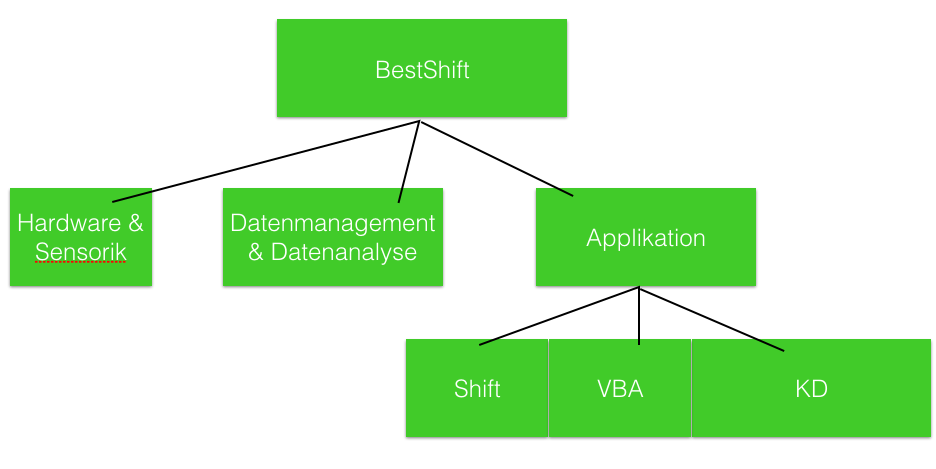
\includegraphics[scale=0.5]{images/Workflowdiagramm.png}

\newline
\section{Workflow des Projektes}
	\subsection{Tobias Perny - Hardware und Sensorik}
	Tobias Perny ist im Projekt wie bereits erwähnt für die Hardware und Sensorik zuständig. 
	Er arbeitet mit einem Raspberry Pi2 Single Board Computer (SBC), auf welchem verschiedene 
	Sensoren direkt montiert sind, welche dann interpretiert werden. 
	Zusätzlich dazu liest der Raspberry Pi2 die OBD-II Motordaten aus stellt diese zur Speicherung bereit.

	\subsection{Daniel Melichar - Datenmanagement und Datenanalyse}
	 
	\subsection{Raphael Simsek - Schaltvorgangsvorschlag}

	\subsection{Hüseyin Bozkurt - Verbrauchsanalyse}
	 Hüseyin Bozkurt ist für die Verbrauchsdarstellung während der Fahrt-
	 und für die retrospektive Verbrauchsanalyse nach der Fahrt zuständig.
	 Diese wird hauptsächlich in Form von Liniendiagrammen geschehen, indem man
	 den Schadstoffausstoß über eine bestimmte Zeit analysiert.
	 In Verbindung mit der Webapplikation, werden diese Informationen mit OpenMap-Daten verbunden und zur schau
	 gestellt.
	 Somit soll eine umweltentlastende Fahrweise nach und nach gefördert werden.
	 Demnach existiert die Option, die analysierte Fahrt auf Facebook mittels OAuth zu teilen, 
	 um Mitbenutzern der App einen Vergleich bieten zu können und - falls es Fragen wie zum Beispiel zu einer Strecke gibt,
	 ihnen durch diese Vergleichswerte genügend Information zu bieten und eine offene Diskussionsrunde zu starten.
	\subsection{Fitim Faiku - Fahrkomfortanalyse}
	 Fitim Faiku stellt die Fahrgastbequemlichkeit eines KFZ während der Fahrt dar.
	 Dies geschieht in Form eines Kamm'schen Kreises, welches die Längs- und Querbeschleunigung anzeigt.
	 Faiku wird für diese Aufgabe die Programmiersprache Java anwenden.
	 Das Framework MPAndroidChart wird ihm dabei behilflich sein.
	 Bei kurvigen Straßen schlägt der Kreis aus, wodurch der KFZ-Fahrer auf eine Geschwindigkeitsanpassung 
	 audiovisuell aufmerksam gemacht wird.
>>>>>>> 44bfd702ec9a19dd5e03de0d417c2ea9aa7a82b6
